\documentclass{beamer}
\usetheme{metropolis} % Use metropolis theme

\title{ECON 3818: Introduction to Statistics with Computer Applications}
%\subtitle
\date{\today}
\author{Kyle Butts}

\definecolor{blue}{RGB}{0,114,178}
\definecolor{red}{HTML}{EB0E09}
\definecolor{yellow}{RGB}{240,228,66}
\definecolor{green}{RGB}{0,158,115}
\definecolor{maroon}{HTML}{AF3335}
\definecolor{purple}{HTML}{7E90B8}

\definecolor{mybackground}{HTML}{ECECEC}
\setbeamercolor{background canvas}{bg= mybackground}

\definecolor{buff-gold}{HTML}{CFB87C}
\definecolor{buff-grey}{HTML}{565A5C}
\definecolor{buff-lightgrey}{HTML}{A2A4A3}
\definecolor{buff-black}{HTML}{000000}

\setbeamercolor{alerted text}{fg=buff-gold!80!black}
\setbeamercolor{frametitle}{bg=buff-black}
\setbeamercolor{title}{fg=buff-grey}
\setbeamercolor{button}{bg=buff-gold}

% Allow to remove indent w/ \begin{itemize}[leftmargin= *]
\usepackage{enumitem}
\setlist[itemize]{label= \textbullet}

% \usepackage[libertine]{newtxmath}
\usepackage{longtable}
\usepackage{booktabs}
\usepackage{enumitem}


\begin{document}

% Title Page ---------------------------------------
\maketitle


% Chapter 20 ---------------------------------------
\section{Chapter 20: Inference about a Population Mean}

\begin{frame}{Conditions for Inference about a Mean}
	
	We've discussed using confidence intervals and tests of significance for the mean $\mu$ of a population
	 
	In general, our analysis relied on two conditions:
	\begin{itemize}
		
		\item The data is from a \textbf{simple random sample} from the population
		
		\item Observations from the population have a \textbf{normal distribution} with a mean, $\mu$, which is generally unknown and a variance $\sigma^2$, which we've been assuming is known. 
		
	\end{itemize}
	
	We'll now talk about the situation where $\mu$ and $\sigma^2$ are both unknown.
	
\end{frame}

\begin{frame}{Important Reminder}
	
	The sample mean variance and standard deviation are provided below:

	\[
		\text{Variance} = \frac{\sigma^2}{n}
	\]
	
	\[
		\text{Standard Deviation} = \frac{\sigma}{\sqrt{n}}
	\]
	
\end{frame}

\begin{frame}{When $\sigma^2$ is Known}
	Whenever we know the population variance, $\sigma^2$, we base confidence intervals and tests for $\mu$ with the z-statistic:

	\[
		Z = \frac{\bar{X}-\mu}{\sigma/\sqrt{n}}
	\]
	\[
		\text{Where } Z \sim N(0,1)
	\]

	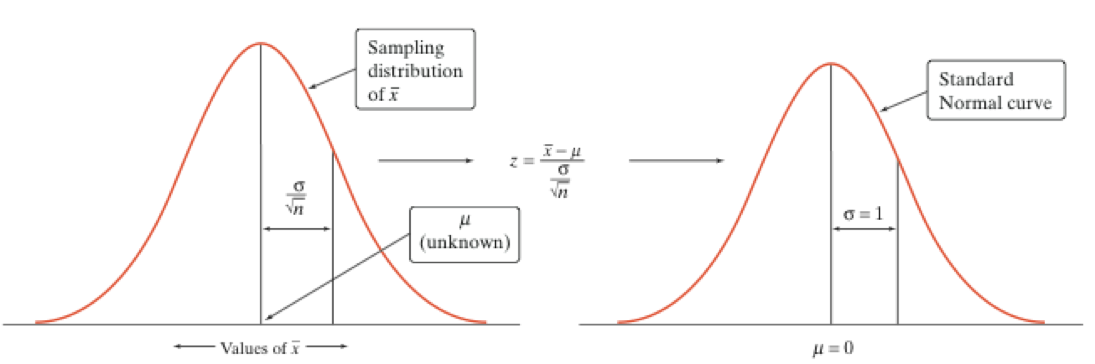
\includegraphics[width=\textwidth]{standard}
\end{frame}

\begin{frame}{When $\sigma^2$ is Unknown}
	When we don't know the true variance, we must use the sample variance $s^2$. Again, since we're talking about sample means, the standard deviation of a sample mean, based of a \textit{population with unknown variance} is:

	\[
		\frac{\sigma^2}{n} \text{ estimated by } \frac{s^2}{n} 
	\]
	\[
		\frac{\sigma}{\sqrt{n}} \text{ estimated by } \frac{s}{\sqrt{n}} 
	\]

	$\frac{s}{\sqrt{n}}$ is called the \alert{standard error}.
	
\end{frame}

\begin{frame}{When $\sigma^2$ is Unknown}
	
	When we don't know $\sigma$, we estimate it by the \textit{sample standard deviation}, $s$. What happens when we standardize?
	$$\frac{\bar{X}-\mu}{s/\sqrt{n}}=???$$
	
	\textbf{This new statistic does not have a normal distribution}
	
\end{frame}

\begin{frame}{The $t$ Distribution}
	
	When we standardize based on the sample standard deviation, $s$, our statistic has a new distribution called a \alert{t-distribution}
	\begin{definition}[t-Statistic and t-Distribution]
		\vspace{5mm}
		Consider a simple random sample of size $n$, the t-statistic:
		\[
			t = \frac{\bar{X}-\mu}{s/\sqrt{n}}
		\]
		has the t-distribution with $n-1$ degrees of freedom
	\end{definition}

	The t-statistic has the same interpretation as z-statistic: it says how far away $\bar{X}$ is from its mean $\mu$, in standard deviation units
	
\end{frame}


\begin{frame}{The $t$-Distribution}
	\begin{itemize}
		\item There is a different $t$ distribution for each sample size, specified by its \alert{degrees of freedom}
			\begin{itemize}
				\item We denote the $t$ distribution with $n-1$ degrees of freedom as $t_{n-1}$
			\end{itemize}

		\item The curve has a different shape than the standard normal curve
			\begin{itemize}
		      	\item It is still symmetric about it's peak at 0
		      	
		      	\item But, it has much more area in the tails.
			\end{itemize}
	\end{itemize}
	
\end{frame}

\begin{frame}{"More Area in the Tails"?}
	\begin{itemize}
		\item Example: 
		
		\begin{itemize}
			\item Let's say I want to predict the height of the class by selecting $n = 3$ people and taking their mean. Sometimes I will pick 3 basketball players or 3 short people.
			
			\item If I am using $n = 20$ people, then it is much more rare to select only tall or only short people (this means the tails are more narrow).
			
			\item I might still select the tallest or shortest person in the class, but they're only one of 20 instead of one of 3.
		\end{itemize}
	\end{itemize}

\end{frame}

\begin{frame}{Graphs of $t$-Distributions}
	\begin{centering}
		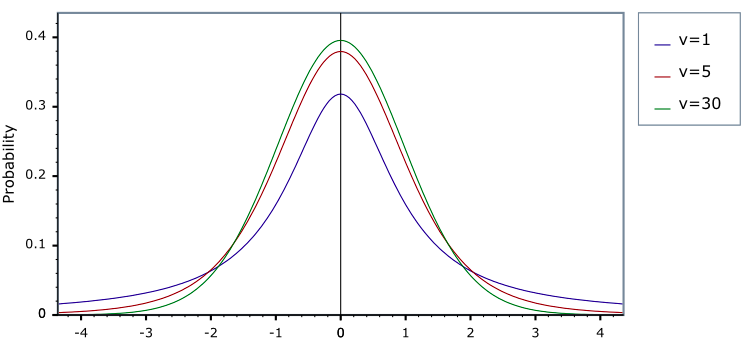
\includegraphics[width=\textwidth]{tdists}
	\end{centering}
\end{frame}


\begin{frame}{Graphs of $t$-Distributions}
	
	\begin{itemize}
		\item Greater degree of dispersion in the $t$ distribution
		      \begin{itemize}
		      	\item it has an additional source of random variability, sample standard deviation $s$
		      \end{itemize}
		\item Sample variance decreases when the sample size increases
		      \begin{itemize}
		      	\item This means the t-distribution looks more like the z-distribution as sample size grows to infinity
		      	\item Once degrees of freedom exceeds 31, the t-distribution is close enough to standard normal  to approximate probabilities using the z-distribution
		      \end{itemize}
	\end{itemize}
	
\end{frame}

\begin{frame}{Finding $t$-values}
	\begin{center}
		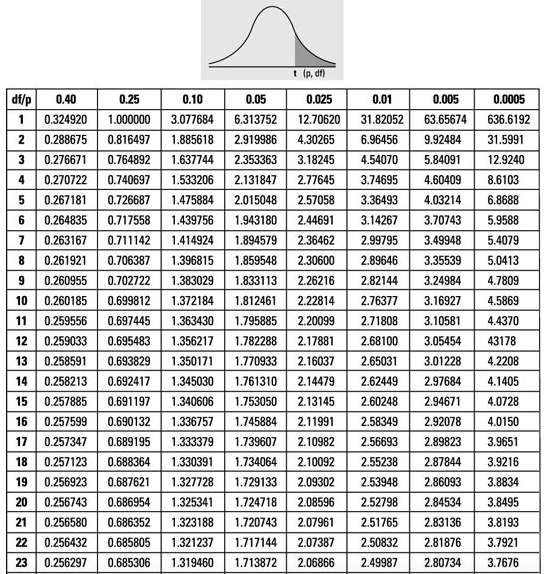
\includegraphics[width=0.75\textwidth]{t_table}
	\end{center}
\end{frame}

\begin{frame}{Finding $t$-values}
	As you see, once we have more than 30 degrees of freedom, we can use the z-scores
	\vskip.25in
	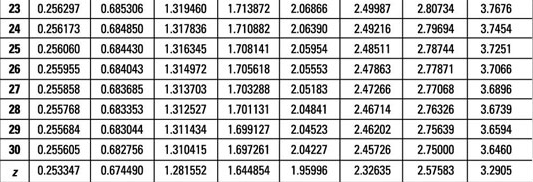
\includegraphics[width=\textwidth]{t_table2}
\end{frame}

\begin{frame}{Confidence Interval with $t$-Distribution}
	Calculating a confidence interval:
	\begin{itemize}
		\item Is variance, $\sigma^2$ known?
		      \begin{itemize}
		      	\item Use Z-distribution
		      \end{itemize}
		\item Is variance $\sigma^2$ unknown?
		      \begin{itemize}
		      	\item 31 or more observations in sample, use Z-distribution
		      	\item 30 or fewer observations inn sample, use t-distribution
		      \end{itemize}
	\end{itemize}
\end{frame}


\begin{frame}{Example}
	Say you want to construct a 95\% confidence interval using 20 observations from population with unknown $\mu$ and $\sigma$, with a sample mean, $\bar{X}=22.21$ and a sample standard deviation, $s=1.963$. 
	
	$\sigma$ is unknown and $n \leq 31 \rightarrow$ use t-distribution:
	
	\[
		CI = \bar{X} \pm t^* \frac{s}{\sqrt{n}}
	\]
	
	\[
		\text{where }t^* = t^\frac{1-C}{2}_{df}=t^{0.025}_{19}
	\]
\end{frame}

\begin{frame}{Example}
	\begin{center}
		Find $t^{0.025}_{19}$ using t-distribution table:

		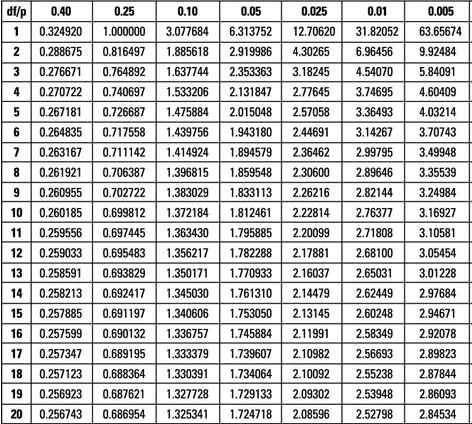
\includegraphics[width=0.6\textwidth]{t_table3}
	\end{center}
	$$t^{0.025}_{19}=2.093$$
\end{frame}

\begin{frame}{Example}
	$$CI = \bar{X} \pm t^* \frac{s}{\sqrt{n}}$$
	$$CI = 22.21 \pm 2.093 \cdot \frac{1.963}{\sqrt{20}}$$
	 
	Which means the confidence interval is [21.29, 23.13].
	
	We are 95\% confident that the population mean is between 21.29 and 23.13.
\end{frame}


\begin{frame}{Clicker Question}
	Which table would you use for the following confidence interval?
	
	\begin{center}
		99\% confidence interval with n=1000 observations
	\end{center}
	\begin{enumerate}[label=(\alph*)]
		\item z-table
		\item t-table

	\end{enumerate}
\end{frame}

\begin{frame}{Clicker Question}
	What critical value $t^*$ would you use for the following confidence interval?
	
	\begin{center}
		90\% confidence interval with n=2 observations
	\end{center}

	\begin{columns}
		\begin{column}{0.3\textwidth}
			\begin{enumerate}[label=(\alph*)]
				\item 2.92
				\item 6.31
				\item 3.08
				\item 1.89
			\end{enumerate}
		\end{column}

		\begin{column}{0.7\textwidth} 
			\begin{center}
			 	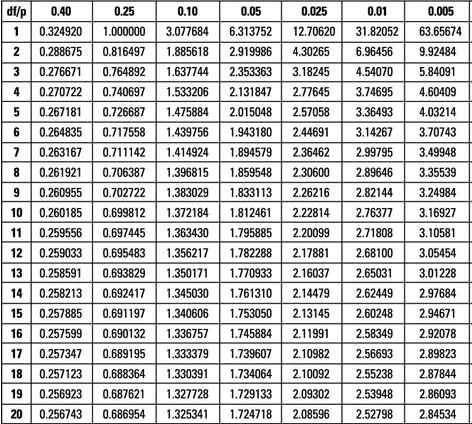
\includegraphics[width=\textwidth]{t_table3}
			\end{center}
		\end{column}
	\end{columns}
\end{frame}

\begin{frame}{Clicker Question}
	What critical value $t^*$ would you use for the following confidence interval?
	
	\begin{center}
		95\% confidence interval with n=16 observations
	\end{center}

	\begin{columns}
		\begin{column}{0.3\textwidth}
			\begin{enumerate}[label=(\alph*)]
				\item 1.753
				\item 1.745
				\item 2.13
				\item 2.12
			\end{enumerate}
		\end{column}

		\begin{column}{0.7\textwidth} 
			\begin{center}
			 	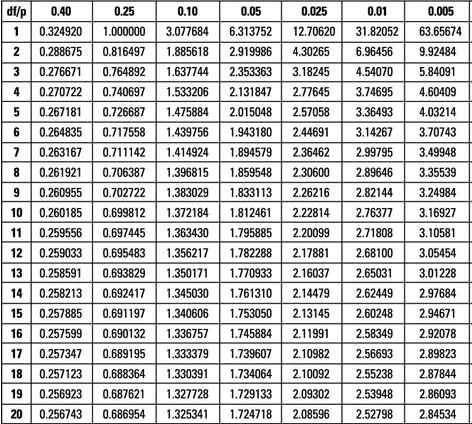
\includegraphics[width=\textwidth]{t_table3}
			\end{center}
		\end{column}
	\end{columns}
\end{frame}


\begin{frame}{Clicker Question -- Midterm Example}
	A randomly sampled group of patients at a major U.S. regional hospital became part of a nutrition study on dietary habits. Part of the study consisted of a 50-question survey asking about types of foods consumed. Each question was scored on a scale from one (most unhealthy behavior) to five (most healthy behavior). The answers were summed and averaged. The population of interest is the patients at the regional hospital. A sample of n = 15 patients produced the following statistics $\bar{X}=3.3$ and $s=1.2$. A 99\% confidence interval is given by:

	\begin{enumerate}[label=(\alph*)]
		\item (2.37, 4.22). %%
		\item (2.64, 3.97).
		\item (2.69, 3.91).
		\item (2.5, 4.1).
	\end{enumerate}
\end{frame}



\begin{frame}{Hypothesis Test with $t$-Distribution}
	Like the confidence interval, the $t$ test is very similar to the $Z$ test introduced earlier.
	
	If we have  SRS of size $n$ from population with unknown $\mu$ and $\sigma$. To test the hypothesis: $H_0: \mu = \mu_0$, compute the \alert{t-statistic}:
	$$t=\frac{\bar{X}-\mu_0}{s/\sqrt{n}}$$
	We then use this t-statistic to calculate the p-value
	\begin{itemize}
		\item The p-values are exact if the population does happen to be normally distributed
		\item Otherwise, they are approximately correct for large enough $n$
	\end{itemize}
\end{frame}


\begin{frame}{p-Values in $t$-Distribution}
	\begin{center}
		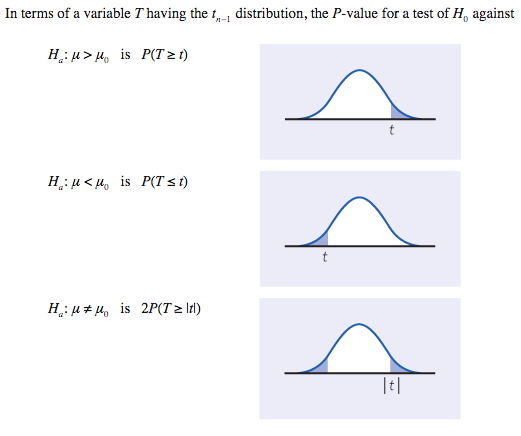
\includegraphics[width=0.8\textwidth]{pvalues_t}
	\end{center}
\end{frame}


\begin{frame}{Example}
	Suppose we have a sample of 12 observations and calculate a sample mean $\bar{X}=113.75$ and a sample standard deviation, $s=93.90$, and we want to test the following hypothesis at the $\alpha=0.10$ level:

	\[ 
		H_0: \mu=88 
	\]
	\[ 
		H_1: \mu > 88 
	\]
	
	The set up is similar to how we've done hypothesis testing before, but we must use the t distribution.
	
	\[ 
		P(\bar{X} > 113.75 \ \vert \ \mu = 88) 
	\]
\end{frame}

\begin{frame}{Example}
	When we "standardize", we are going to be using the t-distribution since we don't know the population variance and we have a small sample. 
	\[ 
		P(\bar{X} > 113.75 \ \vert \ \mu=88) = P(\frac{\bar{X}-\mu_0}{s/\sqrt{n}} > \frac{113.75-88}{93.90/\sqrt{12}})
	\]
	\[ 
		= P(t_{11}>0.95)
	\]
\end{frame}


\begin{frame}{Example}
	Our next step is to find the p-value associated with that t-statistic
	\begin{itemize}
		\item We can pin down the p-value between two points by using the t-table used earlier. 
		      \begin{itemize}
		      	\item Look at the row, df=11
		      	\item See which columns 0.95 lies between, and look at their associated probabilities 
		      \end{itemize}
	\end{itemize}
\end{frame}

\begin{frame}{Example}
	\begin{center}
		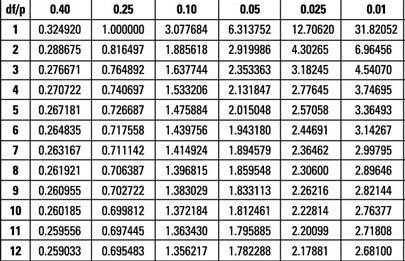
\includegraphics[width=0.65\textwidth]{t_table4}\\
	\end{center}
	We see that along the row with 11 degrees of freedom,  Our t-statistic (0.95) is between 0.25, which has a t-statistic of 0.697, and 0.10, which has a t-statistic of 1.36.\\
	
	We conclude that $0.10 \leq p-value \leq 0.25$
\end{frame}

\begin{frame}{Example}
	Our level of significance is $\alpha=0.10$, and we concluded that the p-value associated with this hypothesis is test is greater than 0.10. 
	
	Therefore:
	
	\[
		\alpha \leq p-\text{value} \implies \text{ Do not reject } H_0
	\]

	That main difference between solving a hypothesis test with z-statistic versus t-statistic is that we will generally only be able to find a range for the p-value with t-statistic, whereas we found an exact value with a z-statistic.
\end{frame}


\begin{frame}{Clicker Question}
	Say we have calculated a $t$-statistic of 1.6 from a sample of 24 observations. Do we reject at the $\alpha=0.10$ level? What about the $\alpha=0.05$ level?
	
	\begin{enumerate}[label=(\alph*)]
		\item Reject at both $\alpha=0.05$ and $\alpha=0.10$
		\item Do not reject at both $\alpha=0.05$ and $\alpha=0.10$
		\item Reject at $\alpha=0.05$, but do not reject at  $\alpha=0.10$
		\item Reject at $\alpha=0.10$, but do not reject at  $\alpha=0.05$
	\end{enumerate}
\end{frame}


\begin{frame}{Hypothesis Testing with t-Distribution}
	When we conduct a hypothesis test we follow these steps:
	\begin{itemize}
		\item Calculate the test statistic
		      $$t=\frac{\bar{X}-\mu_0}{s/\sqrt{n}}$$
		
		\item Determine range of p-values associated with test statistic using t-table
			\begin{itemize}
		      	\item Row is determined by degrees of freedom, $n-1$
		      	\item Find which two columns your t-statistic lies between
			\end{itemize}
		
		\item Similar to hypothesis testing with a Z distribution, if using a two-tailed test, multiply $p$-value by 2.
		
		\item Compare range of p-values to $\alpha$
	\end{itemize}
\end{frame}

\begin{frame}{Example} 
	Collect sample of 12 fish and measure gill length. Calculate $\bar{X} = 3.12$ and $s = 0.7$. Test the following hypothesis at the $\alpha = 0.05$ level:
	\[
		H_1:\mu<3.5
	\]
	\[
		H_0:\mu=3.5
	\]
\end{frame}

% Solve Example
\begin{frame}{Example}
\end{frame}

\begin{frame}{Example}
	Observe sample of 27 newborns in a hospital near Chernobyl and record number of fingers. You calculate $\bar{X} = 9.2$ and $s = 1.8$. You want to test to the following hypothesis at the $\alpha=0.10$ level:
	\[
		H_0:\mu=10
	\]
	\[
		H_1:\mu \neq 10
	\]
\end{frame}

% Solve Example
\begin{frame}{Example}
\end{frame}



\begin{frame}{Rejection Region from $t$-Table}
	
	Lookup the critical value $t^*$, based off the degrees of freedom and level of significance, $\alpha$
	
	\begin{itemize}
		\item Right tailed test:
			\begin{itemize}
		      	\item Reject $H_0$ when $t > t^*$
			\end{itemize}
		      
		\item Left tailed test:
			\begin{itemize}
		      	\item Reject $H_0$ when $t < -t^*$
			\end{itemize}	      
	\end{itemize}
	
\end{frame}


\begin{frame}{Example}
	Suppose you collect a sample of 17 family incomes. You calculate $s = \$6,000$. You want to test the following hypothesis:
	
	\[ 
		H_0: \mu=\$ 29,000
	\]
	\[ 
		H_1: \mu > \$29,000
	\]
	
	If we test at the $\alpha = 0.05$ level, what is our rejection region?
\end{frame}

% Solve Example
\begin{frame}{Example}
\end{frame}


\begin{frame}{Example}
	Suppose you collect a sample of 25 students and record their test scores. You calculate $s=4.2$. If we're testing the following hypothesis:
	\[ 
		H_0: \mu=82
	\]
	\[ 
		H_1: \mu<82
	\]
	If we're testing at the $\alpha=0.01$, when do we reject the null hypothesis?
\end{frame}

% Solve Example
\begin{frame}{Example}
\end{frame}

\begin{frame}{Example}
	Back to our newborn example. Observe sample of 27 newborns in a hospital near Chernobyl and record number of fingers. You calculate $s=1.8$. If we're testing the following hypothesis at the $\alpha=0.05$ level, what is the rejection region?
	\[ 
		H_0:\mu=10
	\]
	\[ 
		H_1:\mu \neq 10
	\]
\end{frame}

% Solve Example
\begin{frame}{Example}
\end{frame}


\begin{frame}{Matched Pairs}
	Often we are interested in seeing if a particular treatment has an effect
	\begin{itemize}
		\item Does pollution impact your exam scores?
		\item Does access to birth control increase female labor force participation rates?
		\item Does taking turmeric improve your focus?
	\end{itemize}
	
	These questions can be solved using a \alert{matched pair design}
	\begin{itemize}
		\item a matched pair design involves making two observations on the same individual, or one observation on two similar individuals.
	\end{itemize}
\end{frame}

\begin{frame}{Matched Pairs}
	If the conditions for inference are met, we can use a one-sample t procedures to perform inference about the \textit{mean difference}
	
	Essentially the paired data include variables that are within-pair differences:
	\begin{itemize}
		\item Example: $X_i$ = Country's labor force before birth-control - Country's labor force after birth control
	\end{itemize}
	In these types of problems:
	\begin{itemize}
		\item the parameter interest, $\mu$, is the true population difference
		\item $s$ is the sample standard deviations of within pair difference
	\end{itemize}
\end{frame}

\begin{frame}{Matched Pairs Example}
	Counselor selects 25 students who enrolled at the same school in seventh and eighth grade to see if their GPAs improved compared to the previous school year, after the school decided to implement mandatory study halls.

	\begin{center}
		\scalebox{0.7}{
		\begin{tabular}{|l|c|c|c|}
			\toprule
			% Head -----------------------------------------
			& & \textbf{Sample} & \textbf{Standard Error} \\
			\textbf{Variable} & \textbf{Sample Mean} & \textbf{Standard Deviation} & \textbf{Estimate} \\ 
			\midrule
	
			% Body -----------------------------------------
			Seventh grade GPA & $\bar{x}_7 = 2.89433$ & $s_7 = 0.51053$ & $SE_7 = 0.10211$ \\ 
			Eighth grade GPA & $\bar{x}_8 = 2.96493$ & $s_8 = 0.57332$ & $SE_8 = 0.11466$ \\ 
			Difference (8th - 7th) & $\bar{x} = 0.07060$ & $s = 0.23495$ & $SE = 0.04699$ \\ 
			\bottomrule
		\end{tabular}
		}
		\end{center}

	She conducts the following hypothesis at $\alpha = 0.05$:
	\[
		H_0: \mu = 0
	\]
	\[
		H_1: \mu > 0,
	\]

	where $\mu$ is the mean change in GPA from 7th to 8th grade.
\end{frame}

\begin{frame}{Matched Pairs Example}
	Calculate p-value of the hypothesis test:
	\begin{itemize}
		\item Calculate t-stat: 
			\[ 
				t = \frac{\bar{X}-\mu}{s/\sqrt{n}} = \frac{0.07-0}{.235/\sqrt{25}} = 1.49
			\]
		\item Calculate range of p-values:

		      Row 24, $t = 1.49$ between 0.10 and 0.05 $\implies$ $0.05 < p < 0.10$.
	\end{itemize}
	
	$p>\alpha$ so she would not reject the null that the mandatory study halls had no effect on grades
\end{frame}

\begin{frame}{Matched Pairs Example}
	Say 16 cows are randomly fed two different diets. Milk production was measured for each of the cows during each of the two diets, so that 32 milk production values were recorded. You find the average within cow difference is 0.7 liters of milk, and the sample standard deviation of the within cow difference is 1 liter. 
	
	Consider the following hypothesis test:
	$$H_0: \mu=0$$
	$$H_1: \mu \neq 0$$
	
	Do we reject the null that the cow's produce the same amount of milk at the $\alpha=0.05$ significance level?
\end{frame}

\begin{frame}{Matched Pairs Example}
	Calculate the p-value of hypothesis test:
	\[ 
		t=\frac{0.7-0}{1/\sqrt{16}}=2.8 
	\]

	$t_{15} = 2.6$ when $\alpha = 0.01$ and $t_{15} = 2.95$ when $\alpha = 0.005$
	
	This means the p-value is in between $2 \cdot (0.005)$ and $2 \cdot (0.01)$ because we are looking at a two-tailed test.
	
	Therefore, $0.01 < p \text{-value} < 0.02$, 
	 
	and we reject the null of no difference because our p-value range is less than $\alpha = 0.05$
\end{frame}

\begin{frame}{Clicker Question -- Midterm Example}
	Which of the following is an example of a matched pairs design?
	\begin{enumerate}[label=(\alph*)]
		\item A teacher compares the pretest and posttest scores of students. %%
		\item A teacher compares the scores of students who had a computer-based method of instruction with the scores of other students who had a traditional method of instruction.
		\item A teacher compares the scores of students in her class on a standardized test with the national average score.
		\item A teacher calculates the average of students' scores on a pair of tests and wishes to see if this average is larger than 80\%.
	\end{enumerate}
\end{frame}


\begin{frame}{When to Use Which Distribution}
	
	If we have SRS, Normal X, and $\sigma$ known:
	\begin{itemize}
		\item Use Z distribution
	\end{itemize}

	If we have SRS, Normal X, and $\sigma$ unknown:
	\begin{itemize}
		\item Use the t distribution
	\end{itemize}

	What if we don't know that X is normal?
	\begin{itemize}
		\item $n<15 \implies$ only use t if X looks very normal
		
		\item $15<n<31 \implies$ use t as long as there are no extreme outliers
		
		\item $n>31$, probably okay using Z
	\end{itemize}
	
	Recall Law of Large numbers that says as $n \to \infty$:
		\[ 
			\frac{\bar{X}-\mu}{\sigma/\sqrt{n}} \to^d Z\sim(0,1)
		\]
	
\end{frame} 

\begin{frame}{Takeaway}
	So we can relax the assumption
	\begin{itemize}
		\item $X$ is normally distributed
		\item $\sigma$ is known
	\end{itemize}
	
	If you don't have a simple random sample, everything changes. 
\end{frame}

\begin{frame}{Additional Examples}
	A special diet is intended to reduce systolic blood pressure among patients diagnosed with stage 2 hypertension. If the diet is effective, the target is to have the average systolic blood pressure of this group be below 150. After six months on the diet, an SRS of 28 patients had an average systolic blood pressure of $\bar{X} = 143$ with standard deviation $s = 21$. Is this sufficient evidence that the diet is effective in meeting the target? If you are testing the null hypothesis that the average is 150 against the alternative that the average is less than 150, what conclusion should you draw at the 5\% level of significance?
\end{frame}

%\begin{frame}{Additional Examples}
%The-sample t statistic from a sample of $n$ = 23 observations for the test of $H_0: \mu = 15$ versus $H_1: \mu > 15$ %has the value \\
%$t$ = 2.24. If the standard deviation from the sample is 2.4, what is the mean of these $n$= 23 observations? Round to nearest whole number.
%\begin{enumerate}[label=(\alph*)]
%\item 14 
%\item 15
%\item 16 %%
%\item The mean cannot be determined from the information given
%\end{enumerate}
%\end{frame}

\begin{frame}{Additional Examples}
	A survey regarding dietary habits was distributed at a hospital. Each question was scored on a scale from one (most unhealthy behavior) to five (most healthy behavior). The answers were summed and averaged. The population of interest is the patients at the regional hospital. The current survey was implemented after patients were subjected to this education, and it produced the following sample statistics for 15 patients sampled: $\bar{X} = 3.3$ and $s = 1.2$. We would like to know if the education improved nutrition behavior. We test the following hypothesis at $\alpha = 0.05$
	\[ 
		H_0: \mu=2.9
	\]
	\[ 
		H_1: \mu>2.9
	\]
\end{frame}

\begin{frame}{Additional Examples}
	Researchers want to determine if using wearable technology helps people lose weight. They have a 23 subjects who they weigh before using the technology and 24 months after using the technology. The differences in weight had $\bar{X} = -3.5$ and $s = 7.8$. Is there significant evidence of a reduction in weight after using the wearable technology? Test at $\alpha = 0.05$ level.
\end{frame}








\end{document}